% \begin{center}

% 	\normalsize{Федеральное государственное автономное образовательное учреждение высшего образования}
	
% 	\textbf{НАЦИОНАЛЬНЫЙ ИССЛЕДОВАТЕЛЬСКИЙ УНИВЕРСИТЕТ \\ «МОСКОВСКИЙ ФИЗИКО-ТЕХНИЧЕСКИЙ ИНСТИТУТ»}
% 	\vspace{13ex}
	
% 	\textbf{Вопрос по выбору \\ Электричество и магнетизм
% 	\\ «Дрейф заряженной частицы в неоднородном магнитном поле при наличии слабого
% 		электрического поля» }
% 	\vspace{40ex}
	
% 	\normalsize{Панферов Иван Алексеевич \\ студент группы Б01-001\\ 2 курс ФРКТ\\}
% 	\end{center}
	
% 	\vfill
	
% 	\begin{center}
% 	г. Долгопрудный\\
% 	2021 г.
% 	\end{center}

% \newpage

% \tableofcontents

% \newpage

\section{Электрический дрейф}

Как выяснено выше, в первом приближении неоднородность электрического 
поля учитывать не надо. Не надо учитывать и неоднородность магнитного поля, 
так как она может сказаться на скорости электрического дрейфа лишь во 
втором приближении. Поэтому можно воспользоваться формулой:

\begin{equation}
	\upsilon_\text{д} = \frac{c}{B^2} [\mathbf{E_\perp}, \mathbf{B}] = \frac{c}{B^2} [\mathbf{E}, \mathbf{B}]
	\label{86.3a}	
\end{equation}

и для 
неоднородных полей. Однако в этом случае формула (\ref{86.3a}) уже не 
будет точной, она дает скорость электрического дрейфа только в первом приближении. 
\

Происхождение электрического дрейфа и аналогичного дрейфа,
вызванного любой малой возмущающей силой $\mathbf{F}$, наложенной на 
магнитное поле, легко понять из следующих соображений. Предполагая
магнитное поле $\mathbf{В}$ однородным, рассмотрим проекцию траектории 
частицы на плоскость, перпендикулярную к этому полю. Примем эту
плоскость за плоскость рисунка, направив магнитное поле к читателю
(рисунки \ref{197} и \ref{198}). В отсутствие электрического поля проекцией
траектории частицы будет окружность ларморовского радиуса $\rho$.

\begin{figure}[h!]
	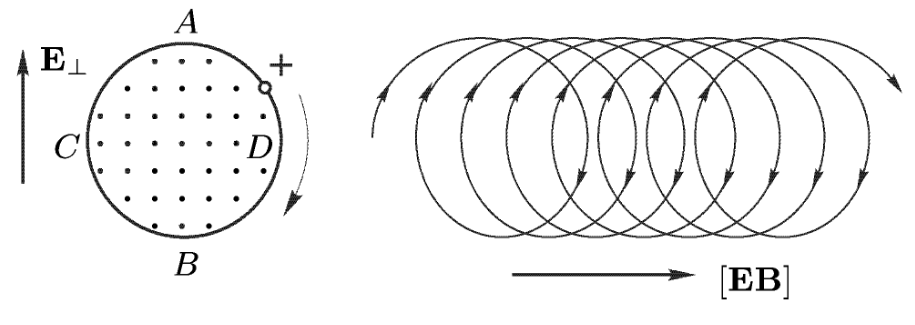
\includegraphics[scale=0.4]{197.png}
	\centering
	\caption{}
	\label{197}
\end{figure}

\begin{figure}[h!]
	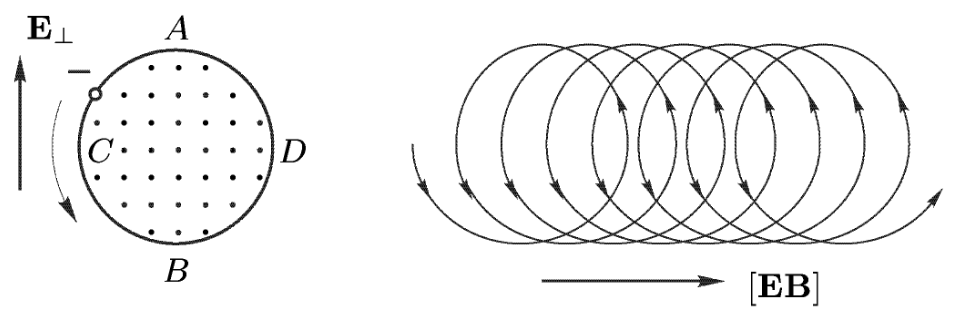
\includegraphics[scale=0.4]{198.png}
	\centering
	\caption{}
	\label{198}
\end{figure}

Для определенности будем иметь в виду движение положительно
заряженной частицы (рис. \ref{197}). Наложим теперь электрическое поле, 
составляющая $\mathbf{E}_\perp$ которого направлена вверх. Так как при перемещении
частицы вверх поле $\mathbf{E}_\perp$ совершает над ней положительную работу,
то скорость частицы $\mathbf{v}_\perp$ в верхнем положении \textit{A} будет больше, чем
в нижнем положении \textit{В}. Кроме того, в точке \textit{A} силы электрического
и магнитного полей действуют на частицу в противоположные стороны,
а в точке \textit{В} — в одну и ту же сторону. Оба эти обстоятельства приводят
к тому, что радиус кривизны \textit{r} проекции траектории в верхней части
увеличивается, а в нижней уменьшается, как это видно из выражений

\[
    \frac{1}{r} = \frac{eB}{m \upsilon_\perp c} - \frac{eE_\perp}{m\upsilon_\perp^2} ~~~~ \text{(в точке \textit{A}),}
\]

\[
    \frac{1}{r} = \frac{eB}{m \upsilon_\perp c} + \frac{eE_\perp}{m\upsilon_\perp^2} ~~~~ \text{(в точке \textit{B}).}
\]

В результате окружность перейдет в незамкнутую кривую, двигаясь
по которой проекция частицы будет медленно перемещаться вправо
(рис. \ref{198}, справа). Это перемещение и есть электрический дрейф. Для
отрицательно заряженной частицы аналогичное перемещение
представлено на рис. \ref{198}. В обоих случаях частица дрейфует вправо, т. е.
направление электрического дрейфа, как это и должно быть, не
зависит от знака заряда частицы.
\

Скорость электрического дрейфа легко определить из следующих
соображений. В положениях \textit{С} и \textit{D} (рис. \ref{198}) частица движется с одной
и той же скоростью $\mathit{\upsilon}_\textit{С}$, которая больше скорости частицы в нижнем
положении \textit{В} и меньше скорости ее в верхнем положении \textit{А} на одну и ту
же величину \textit{u}. Величина \textit{u} и есть скорость электрического дрейфа:
$u = \upsilon_\text{д}$.
Действительно, если ввести систему отсчета, движущуюся вправо со скоростью \textit{u},
то в этой системе скорости частицы в положениях \textit{A} и \textit{B}
сравняются, и частица будет равномерно вращаться по окружности.
Величину \textit{u} определим из уравнения энергии: 
$m(\mathit{\upsilon}_\textit{С} + \textit{u})^2/2 - m\mathit{\upsilon}_\textit{С}^2/2 = eE_\perp \rho$.
Подставляя сюда $\rho = mc\mathit{\upsilon}_\textit{С}/(eB)$ и пренебрегая квадратом
скорости \textit{u}, получим
$$\upsilon_\text{д} = u = \frac{E_\perp}{B}c \text{.}$$
что совпадает с формулой (\ref{86.3a}).

% \begin{thebibliography}{3}
% 	\bibitem{1}	Д.В.Сивухин <<ОБЩИЙ КУРС ФИЗИКИ>> Том III Электричество и Магнетизм
% \end{thebibliography}
